\section{Les supernovae}



\subsection{le modele theorique}
il existe principallement deux evenement pouvant mener a un explosion de supernovae : 

\begin{itemize}
\item soit l'étoile est a l'origine suffisemant massive (plus de 8Mo) pour s'effondrer a la fin de sa vie.
\item soit l'etoile n'est pas suffisement massive (elle va donc mourrir en naine blanche) mais dispose de suffisement de matière a proximité (générallement étopiles double ou le compagnon pas en phase géante rouge) pour que sa masse augmente avec le temps.
la matière acretté va faitre passer la masse de cettte étoile au dessu de la limite.
\end{itemize}






Les etoiles de plus de 8mo ewploses en SN en injectant 1e51 erg dans le milieu\\
Cette injection limite fortement la formation stellaire dans le milieu.\\
modele sous grille\\



Les differentes phases
\begin{itemize}
\item expansion adiabatique
\item snowplow
\end{itemize}

Dans la phase d'expansion adiatique, l'energie est conservé, le choc est violent et le gas n'a pas le temps de perdre de l'energie par radiation.
Dans la phase snowplow, le choc a suffisemment ralentis pour que le gas commence a rayonner de l'energie, l'energie n'est plus conservée.


\subsection{les superbubles}
Dans les endroits de formation stellaire, les étoiles ne sont pas isolées mais apparaisent ensemble au sein d'un même nuage de gas.
L'effondrement gravitationnel du nuage mêne a créer un génération d'etoile en un cours laps de temps.
Toutes ces étoiles vont mourrir dans un laps de temps rapproché et ainsi, les differentes supernovae vont injectée de l'energy dans le milieu dans un temsp tres rapproché.
Les différentes bulle vont se rencontrer (a la manière des bulles ionizées) en mener a une bulle plus grande appelée superbuble.


\subsection{les considerations d'echelles}
La facon de gerer les supernovae sera donc fonction de léchelle que l'on considere.
Dans des simulations tres detaillées de galaxies, il sera necessaire de resoudre la phase adiabatique d'explosion individuelle.
Dans des simulations cosmologiques de la reionisation, l'interet sera plus porté sur la phase snowplow des superbubbles.


\subsection{ differentes implementations existantes}


\subsection{le model thermique}
Le model thermique consiste a injecter l'energie sous forme d'energie interne.
Il existe 2 variables d'etat liées a l'energie interne: la pression et la température.
Modifié l'une de ses 2 variables est equivalent.

Dans l'implementation actuelle, la pression est modifiée en utilisant cette conversion:

\begin{equation}
P^{0+} = P^{0-}  + E_0 * (\gamma-1)
\end{equation}



\subsubsection{le model cinetique}

Le model cinetique consiste a modifiée la vitesse du gaz autour de l'explosion.
Nous avons fait le choix de limiter le nombre de cellules utilisées a 8 correspondant a 1 oct de la structure AMR d'\emma


\begin{equation}
e_{SN} = E_{SN}/8
\end{equation}

Then this energy is used to change the gas velocity by using:
\begin{equation}
    \Delta \overrightarrow{v_{gas}} = \sqrt{\frac{2e_{SN}}{\rho_g.dV}} \overrightarrow{u}
    \label{eq_sn_direct}
\end{equation}


\subsection{Test numérique (Sedov)}

la derivation des solutions du test de Sedov se trouve :
chapitre 17 de Shu the physique of astrophysic Volume 2.\\

Le test de Sedov cherche a reproduire une explosion parfaite.
Il consiste a relacher instantanemant une quantité dénergie $E_0$ dans un milieu homogène d'indice adiabatique $\gamma$, de densité $\rho_0$ et de pression $P_0$ (ou de température $T_0$).

Sedov a demontré en 1959 que :

\begin{equation}
r_{(t)}=\left( \frac{E_0}{\alpha \rho_0 }\right)^{1/5} t^{2/5}
\end{equation}



Ce brusque changement dans l'etat du systeme créer une discontinuité que le solveur va devoir gérer.


\subsubsection{Sedov Setup}

parametre du test :
rho=1
p=1e-5
v=0
gamma=5/3

\subsubsection{Sedov evolution}

injection thermique simple\\
test en 256**3 sans raffinement\\

\begin{figure}[bth]
        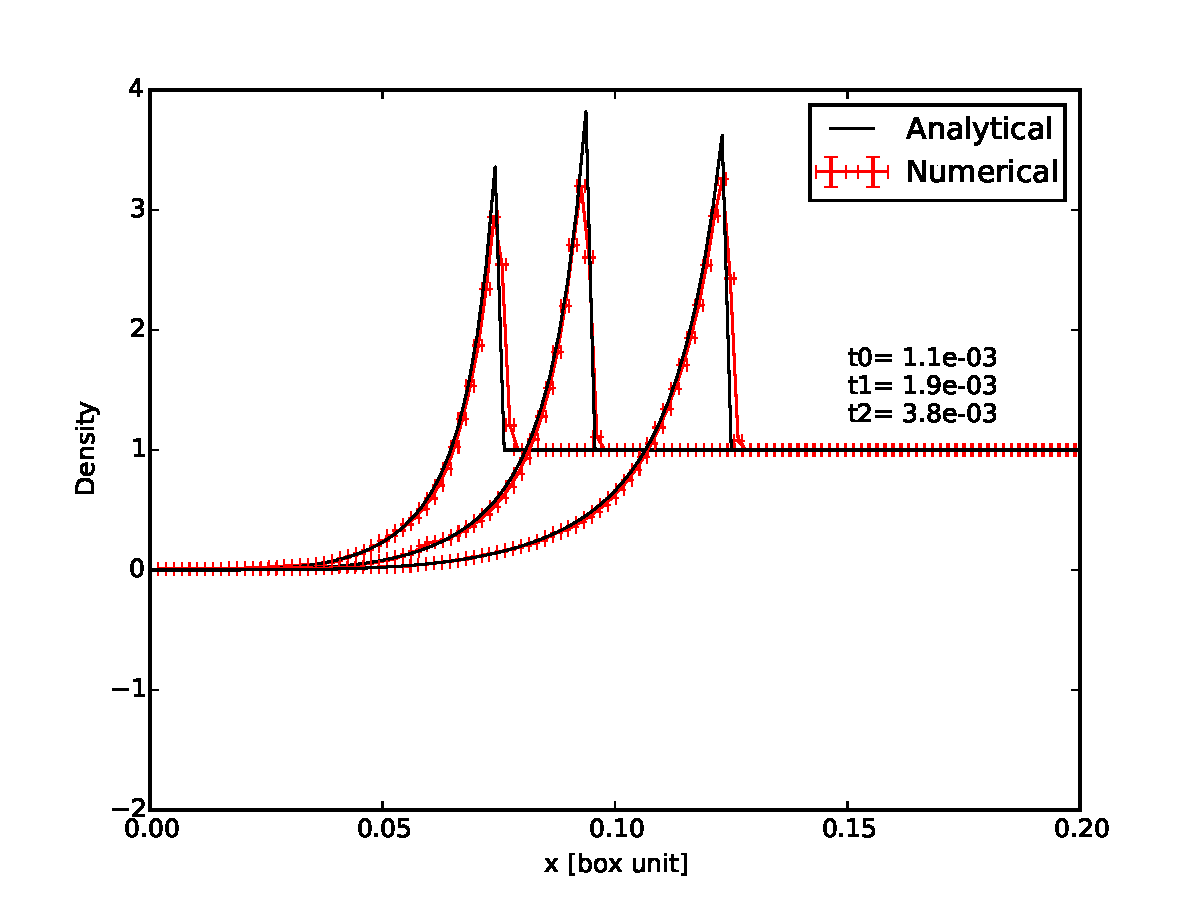
\includegraphics[width=.95\linewidth]{img/03/sedov/sedov_evol_8_den_lin.pdf} 
		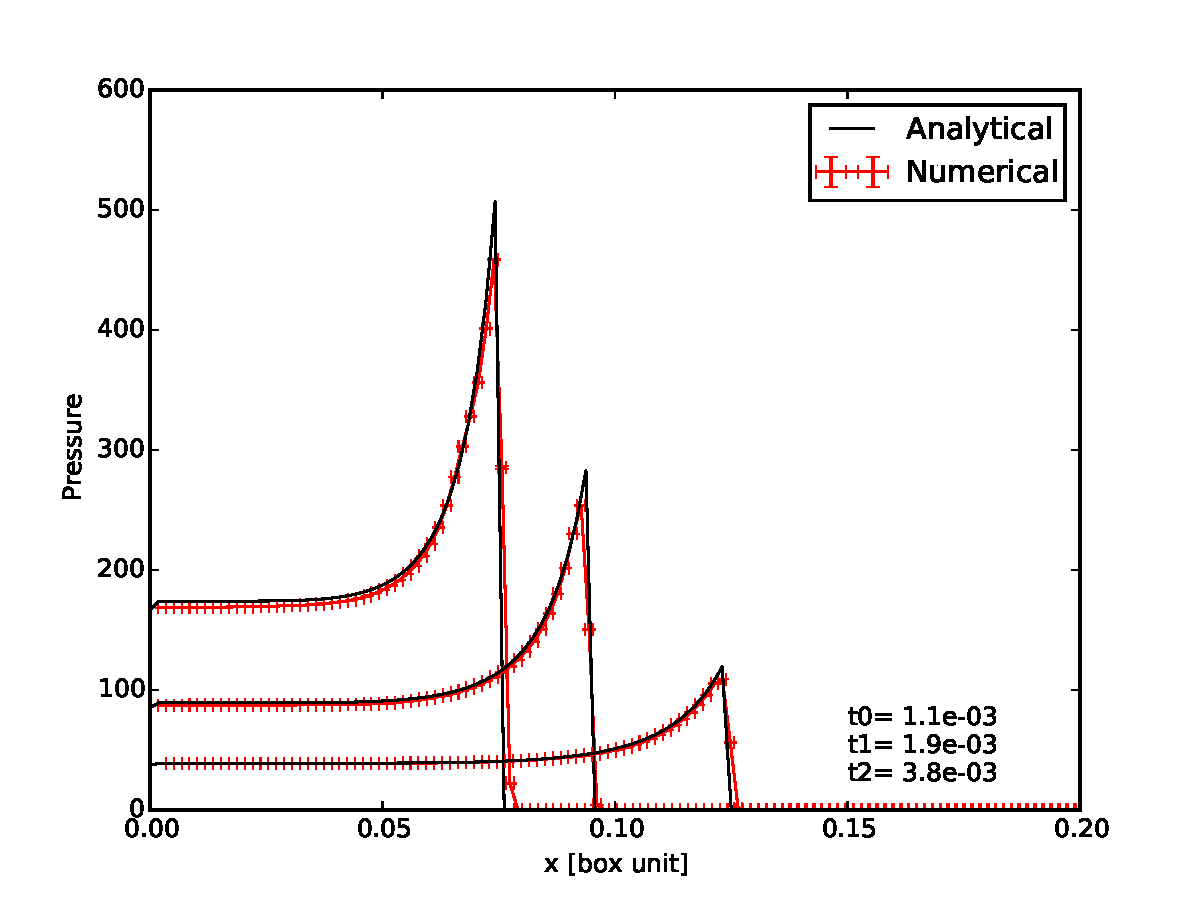
\includegraphics[width=.95\linewidth]{img/03/sedov/sedov_evol_8_pres.pdf} 
		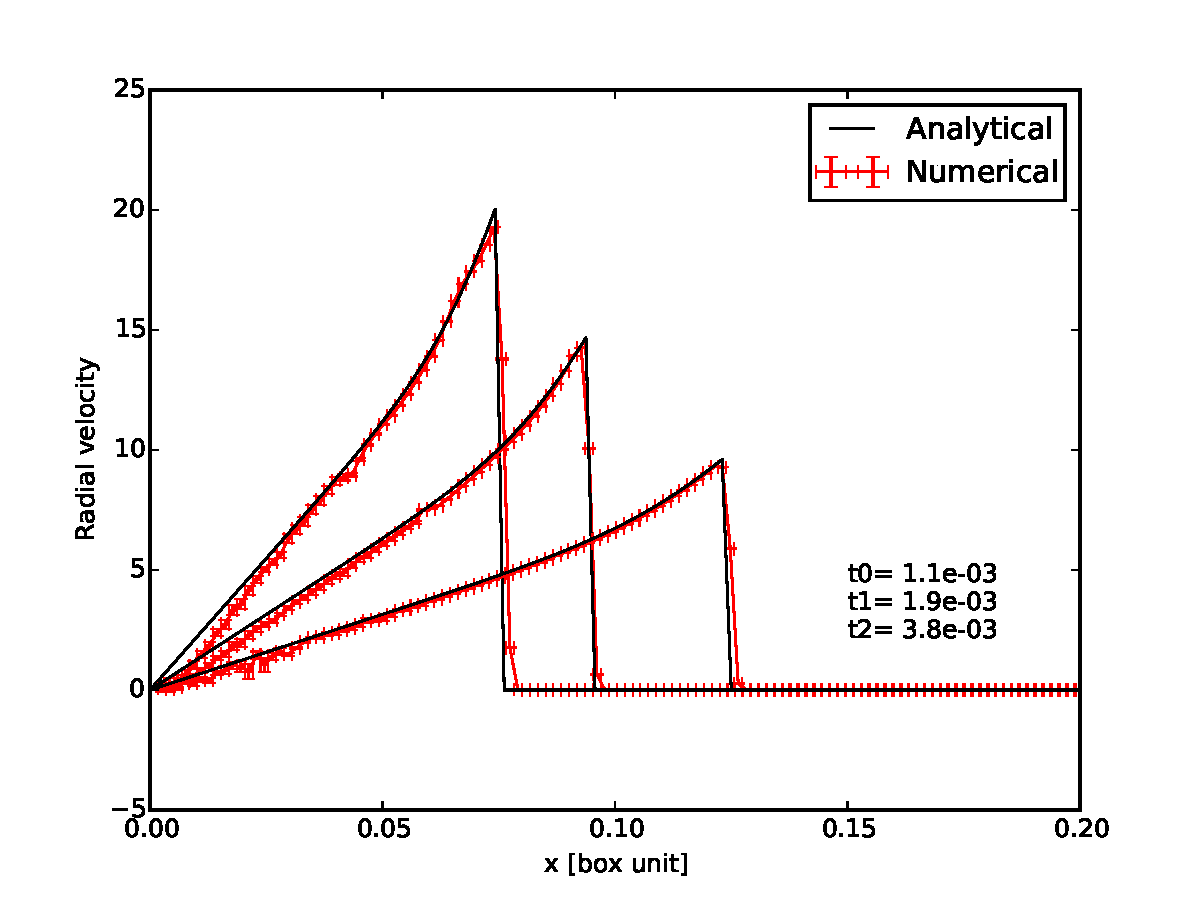
\includegraphics[width=.95\linewidth]{img/03/sedov/sedov_evol_8_vel.pdf} 
        \caption{Test de Sedov, evolution des differentes variables d'etats}
 		\label{fig:}
\end{figure}


\subsubsection{Sedov comparaison}

test en 128**3 avec raffinement, 3 niveaux

mise en place du raffinement :
raffinement sur le gradient 

\begin{figure}[bth]
        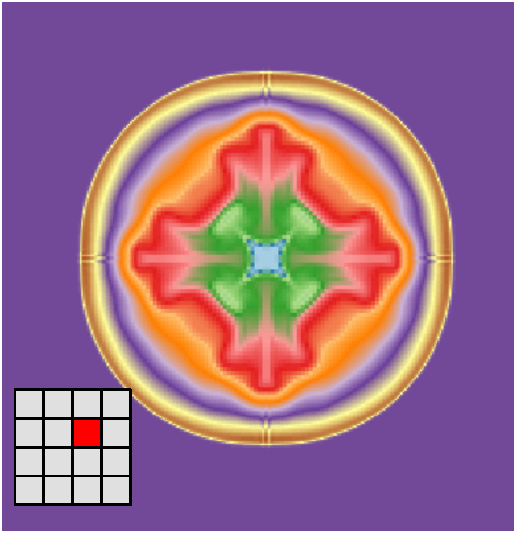
\includegraphics[width=.95\linewidth]{img/03/sedov/slice_therm1.pdf} 
		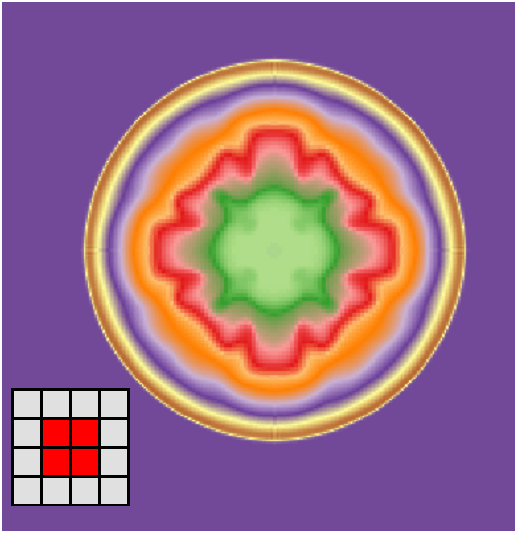
\includegraphics[width=.95\linewidth]{img/03/sedov/slice_therm4.pdf} 
		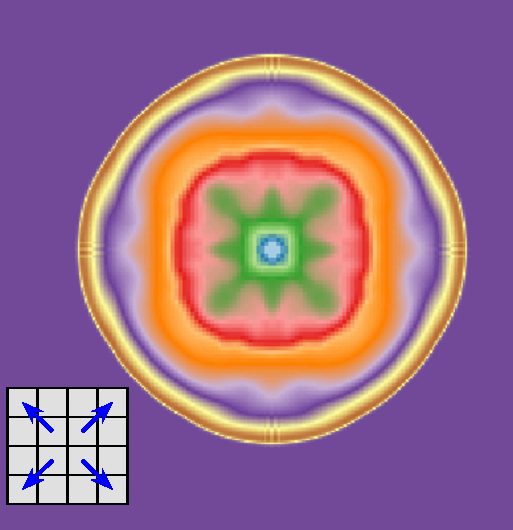
\includegraphics[width=.95\linewidth]{img/03/sedov/slice_kin.pdf} 
        \caption{Test de Sedov}
 		\label{fig:}
\end{figure}

\begin{figure}[bth]
        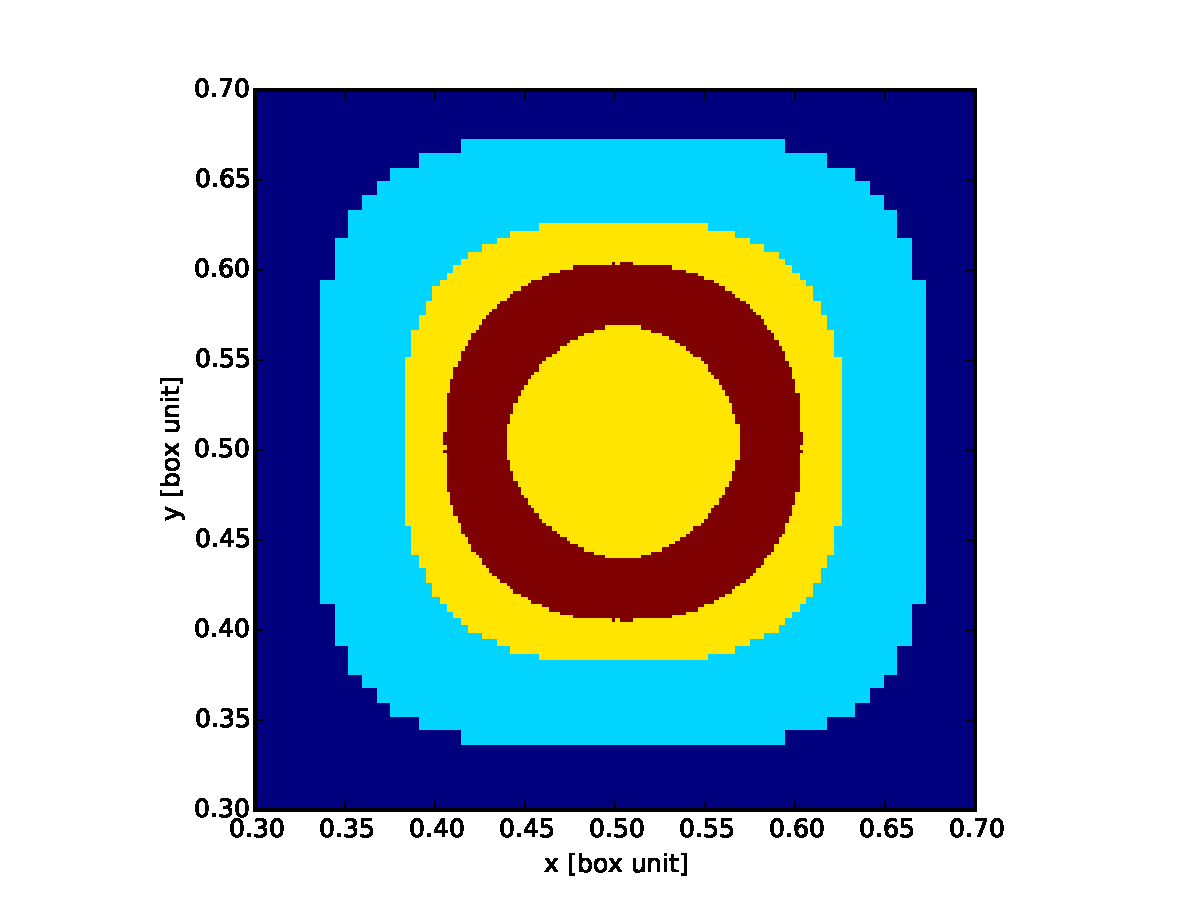
\includegraphics[width=.95\linewidth]{img/03/sedov/slice_th_1raf.pdf} 
        \caption{Test de Sedov, raffinement (mettre la color map) }
 		\label{fig:}
\end{figure}

\begin{figure}[bth]
        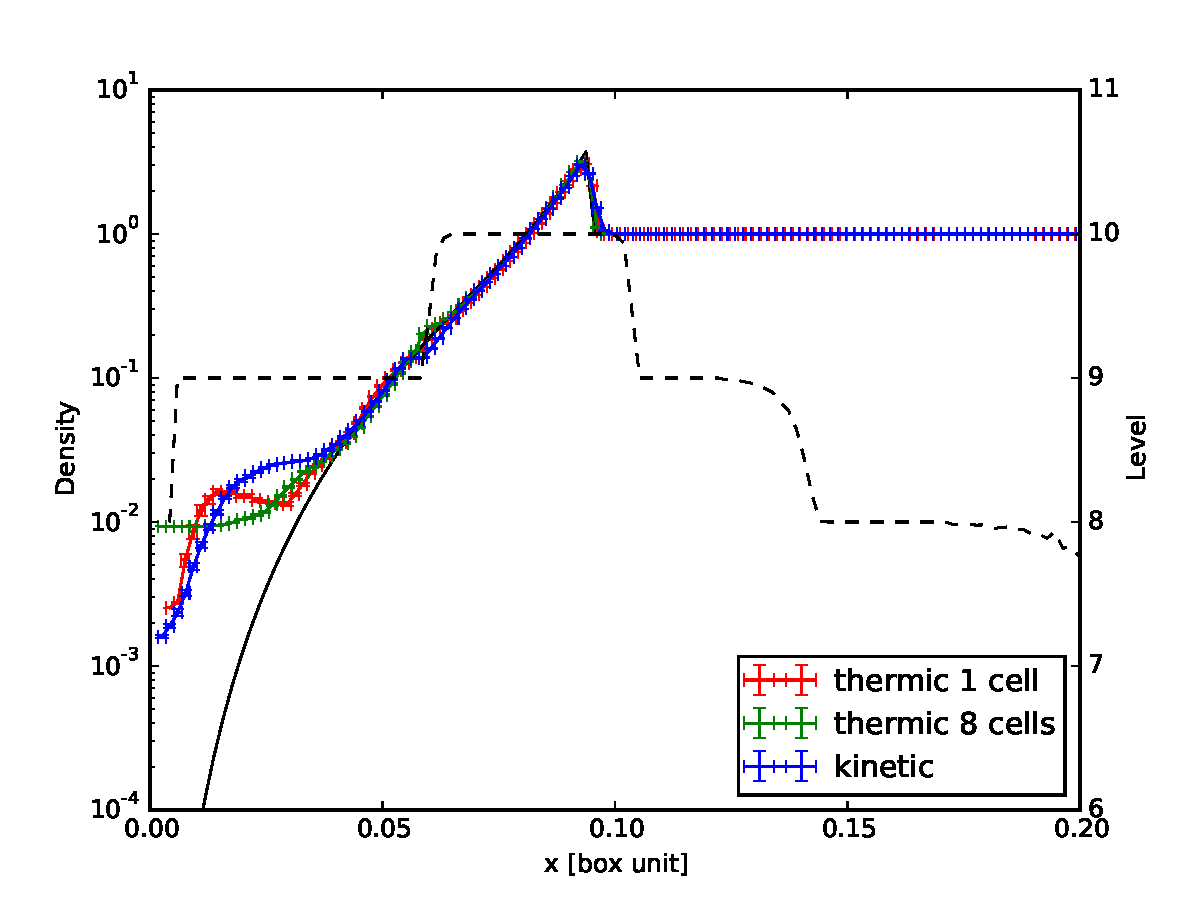
\includegraphics[width=.95\linewidth]{img/03/sedov/sedov_comp_profile_den.pdf} 
		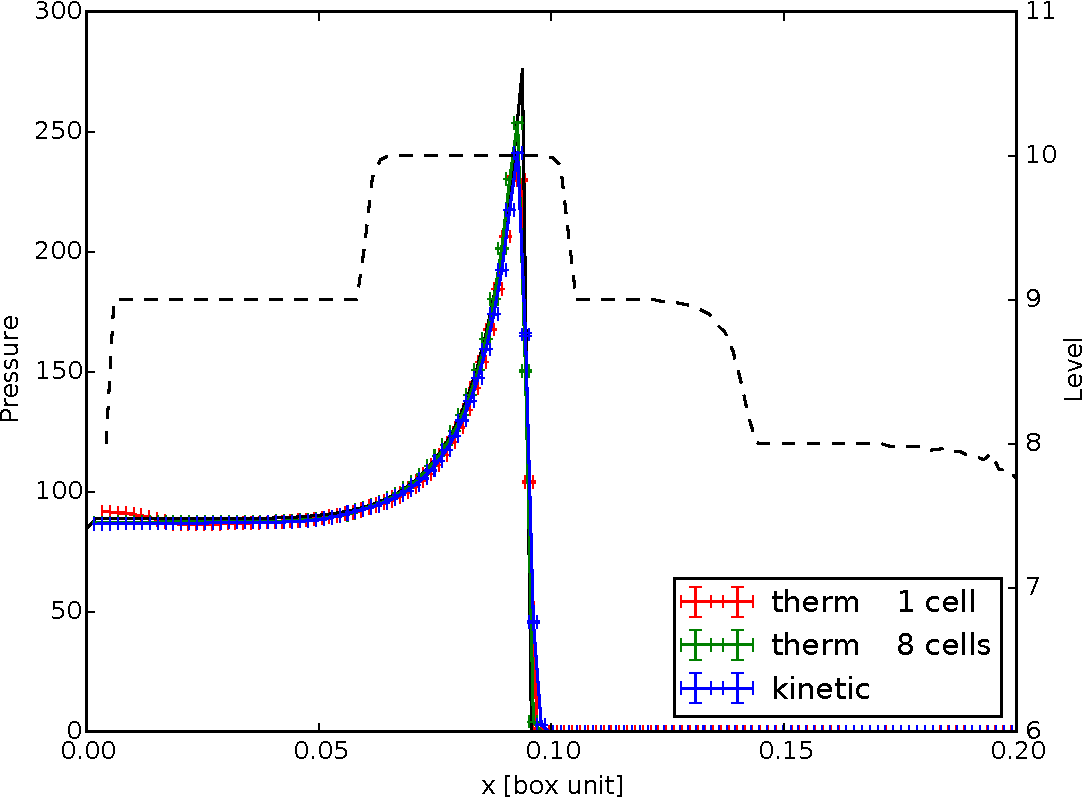
\includegraphics[width=.95\linewidth]{img/03/sedov/sedov_comp_profile_pres.pdf} 
		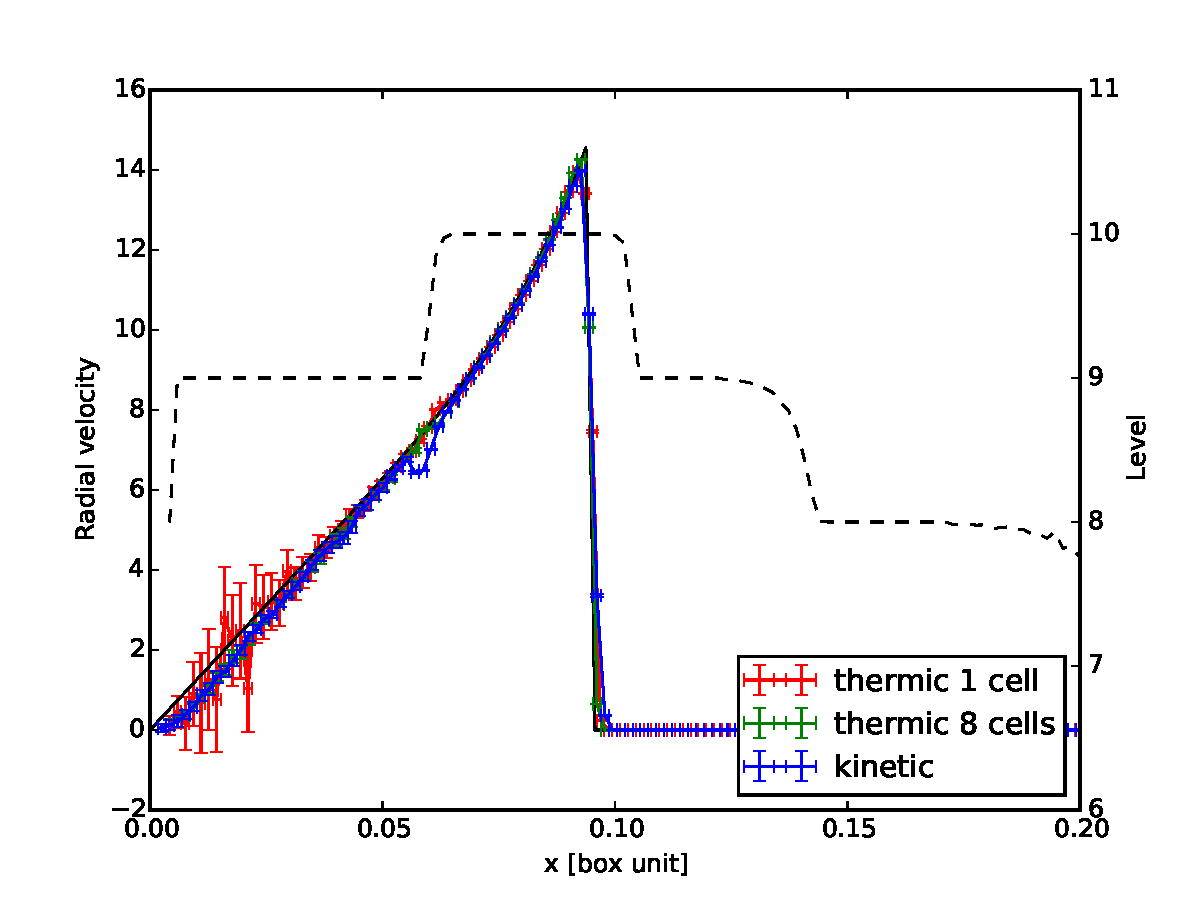
\includegraphics[width=.95\linewidth]{img/03/sedov/sedov_comp_profile_vel.pdf} 
        \caption{Test de Sedov, evolution des differentes variables d'etats}
 		\label{fig:}
\end{figure}


OK\\
mais pas en cosmo

\subsection{Mes Implémentations}



le pas de temps\\
\section{test}
fonction de luminosité 
